\section{High-Level Synthesis}
\label{bg:sec:high_level_synthesis}

High-level synthesis (HLS) is the process of compiling a high-level
representation of an application (usually in C, C++ or MATLAB) into a
register-transfer-level (RTL) implementation~\cite{coussy, gajski}.  In
turn, this RTL design can be synthesized into a circuit and programmed onto
the FPGA device.  With modern HLS tools, some applications synthesized
with them now have similar performance when compared with hand-crafted RTL
implementations~\cite{bdti}.

The major advantage of HLS tools is that they enable us to work in a high-level
language (HLL), as opposed to facing labor-intensive tasks such as optimizing
timing and designing control logic in the RTL design process.  This allows
application designers to focus instead on the algorithmic and functional
aspects of their implementation~\cite{coussy}, without concerning themselves
with the above intricate details of manual RTL designs.

Another advantage of using HLS tools is that they are in general more
productive and less error-prone to work with, when compared with traditional
RTL tools.  The reasons are two-fold.  First, a C description is smaller than
a traditional RTL description by a factor of 10~\cite{coussy, bdti}.  Second,
RTL design can be notoriously difficult to debug, whereas C code can be easily
tested on an ordinary microprocessor, and mature debug and analysis tools for C
are freely accessible~\cite{canis13}.

HLS tools further benefit us in their ability to automatically search
the design space with a reasonable design cost~\cite{bdti}, potentially
explore a large number of trade-offs between performance, cost and
power~\cite{mcfarland}, which is generally much more difficult to achieve
in RTL tools.  Our thesis proposes a natural extension to HLS tools by
automatically exploring the space of rewrites of floating-point numerical
C programs, which are equivalent in real arithmetic, but could trade off
accuracy, throughput and resource utilization when synthesized into circuits.

With recent advancements in this area, HLS tools have received a resurgence
of interest.  Many commercial tools are released, such as Catapult
High-Level Synthesis~\cite{catapultc}, Impulse C~\cite{impulsec} and
PICO~\cite{schreiber02}, to meet the burgeoning demand from the FPGA community.
Xilinx incorporates a sophisticated HLS flow for C/C++ named Vivado HLS into
its Vivado design suite~\cite{vivado_hls}, and their SDAccel Development
Environment~\cite{sdaccel} for C/C++/OpenCL allows data centers to leverage
FPGAs.  Altera's HLS solution is their Altera SDC for OpenCL~\cite{aoc} which
accelerates OpenCL applications on their FPGA devices.  Besides commercial
tools, many open-source HLS tools have also been released in recent years, such
as ROCCC~\cite{roccc}, Trident~\cite{tripp05} and LegUp~\cite{legup}, and LegUp
is now gaining significant traction in the research community.


\subsection{HLS Design Flow}
\label{bg:sub:hls_design}

In this section, we provide an overview of the stages taken by HLS tool to
compile a C program into RTL implementation, by using LegUp~\cite{legup,
canis13} as our example.  LegUp is an HLS tool which compiles programs to run
on a hybrid software/hardware architecture, and its design flow is shown in
Figure~\ref{bg:fig:legup}, which consists of three major stages to be explained
below.
\begin{figure}[ht]
    \centering
    \includegraphics[width=0.7\linewidth]{bg/fig/legup}
    \caption{%
        The LegUp design flow, adapted from~\cite{canis13} and~\cite{legup}.
    }\label{bg:fig:legup}
\end{figure}

The first stage is to determine which parts of an application on the
function-level are suitable candidates to be synthesized into hardware
circuits, while the rest can be run on a processor.  This stage starts by
compiling a C source program into a software executable targeting an FPGA-based
MIPS processor.  This processor has additional circuitries designed to profile
the software implementation of the original application.  By running the
compiled application on this processor, this profiling ability allows the
processor to use statistics such as number of clock cycles, power and cache
misses to identify parts of the program at the function level that will benefit
from a hardware redesign, so that the power efficiency and run time could be
improved~\cite{canis13}.

After identifying functions of the application to be implemented as part
of a hardware architecture, the next stage is then to synthesize hardware
designs from these functions.  LegUp's synthesis toolchain is based on the
low-level virtual machine (LLVM) compiler infrastructure~\cite{llvm}, and it
synthesizes C functions into circuits in a series of steps.

It starts by using the LLVM front-end to compile a C function into LLVM IR,
a platform-independent intermediate representation (IR) that is capable of
cleanly representing HLLs~\cite{llvm_ir}, conventional and HLS-focused compiler
optimization passes are used to transform the IR program, such that the result
when synthesized will have better performance when running on the FPGA\@.

This is then followed by the HLS tool flow, which consists of four logical
steps: allocation, scheduling, binding and RTL generation.  The first
step, allocation, extracts information from the application and user
requirements to be used in subsequent stages, \eg~modules and RAM blocks to be
synthesized on the target device.  This is then followed by scheduling, which
assigns the start and end states to each LLVM instruction in a finite state
machine~\cite{legup}, using a scheduling algorithm based on the formulation
of \emph{system of difference constraints} (SDC)~\cite{legup, canis13,
cong06}.  Many applications spend most of their time in loops, a scheduling
technique, known as \emph{loop pipelining}, is therefore used in HLS tools
to make them run efficiently.  This technique admits greater parallelism of
computation by allowing instructions in consecutive loop iterations to overlap
as much as possible.  LegUp uses an algorithm, known as \emph{modulo SDC
scheduling}~\cite{canis14}, which we will cover in Section~\ref{bg:sub:sdc},
to minimize the wall-clock time of a pipelined loop.  The third logical
step, binding, assigns each operator in the program to functional units to
be synthesized into hardware, and maps program variables to registers.  The
rationale behind this step is that operators such as multipliers and dividers
that tend to use a lot of LUTs and DSP blocks can be shared temporally.
Sharing these functional units requires multiplexers, which is relatively
expensive to implement in FPGA\@.  Each assignment of an operator to a
functional unit is thus associated with a cost.  The problem of minimizing this
cost is called the assignment problem, which is efficiently solved in LegUp
with a polynomial time complexity using the Hungarian algorithm~\cite{canis13,
kuhn10}.  Finally, the RTL generation step gathers information produced from
the previous three steps, to generate Verilog source code corresponding to the
C function being compiled.

The third, and also the final stage, is to integrate software and hardware
components of the application onto the FPGA device, which is explained as
follows~\cite{canis13}.  Firstly, custom accelerator circuits generated by HLS,
a MIPS processor and communication interfaces between them are synthesized
and programmed into the FPGA device.  Because some of the functions in the
original C source code were implemented as hardware accelerators in the HLS
compilation flow, LegUp replaces them with wrapper functions which can invoke
the hardware accelerators in runtime.  Finally, this modified source code can
then be compiled into a MIPS binary to be executed on the FPGA\@.


\subsection{Loop Pipelining}
\label{bg:sub:pipelining}

Loop parallelism, and subsequently, program run time is part of the main
optimization objectives we optimize later in Chapter~\ref{chp:latopt}, hence
in this subsection we first introduce the concept of loop pipelining.  We
consider our example program in Figure~\ref{bg:lst:dotprod}, which computes the
dot-product, \verb|d|, of two arrays \verb|A| and \verb|B| of floating-point
values.  We assume both arrays are stored in the same RAM, which has one read
port, and accessing this RAM has a one cycle latency.  We further assume
no limits on the number of arithmetic operators that can by allocated,
floating-point multiplier and adder are both fully pipelined, and use $7$ and
$10$ cycles respectively to produce outputs.
\begin{figure}[ht]
    \centering
    \begin{minipage}{0.7\textwidth}
    \begin{lstlisting}
    #define N 1024
    float dotprod(float A[N], float B[N])
    {
        float d = 0.0f;
        for (int i = 0; i < N; i++)
        {
            d = d + A[i] * B[i];
        }
        return d;
    }
    \end{lstlisting}
    \end{minipage}
    \caption{%
        A simple dot-product example which calculates the dot-product of two
        arrays \texttt{A} and \texttt{B}, each with 1024 elements.
    }\label{bg:lst:dotprod}
\end{figure}

A trivial way to schedule the loop in Figure~\ref{bg:lst:dotprod} is to allow
each iteration to complete before starting the next iteration; this is however
not very efficient.  As we can see in Figure~\ref{bg:fig:schedule}, with a
good schedule, operations across loop iterations can often temporally overlap,
giving way to parallelism and improve performance of the loop execution.  In
Figure~\ref{bg:fig:schedule}, iterations are laid out in rows, each clock cycle
is a column, \textbf{mul} and \textbf{add} are multiplication and addition
respectively, \verb|A[0]| and \verb|B[0]| are reads from the two arrays, and
the arrows indicate the data-flow of \verb|d| across iterations.  This schedule
allows consecutive iterations to start every 10 cycles; and this number of
clock cycles between the start of consecutive iterations is known as the
\emph{initiation interval} ($\II$).  Loop iterations in this schedule repeat
for $1024$ times (the \emph{trip count}, $N$), and each iteration requires $19$
cycles (the \emph{depth}, $D$, of the loop), as a result the overall latency
$L$ of this loop is $(N - 1) \times \II + D = (1024 - 1) \times 10 + 19 =
10,249$ cycles.
\begin{figure}[ht]
    \centering
    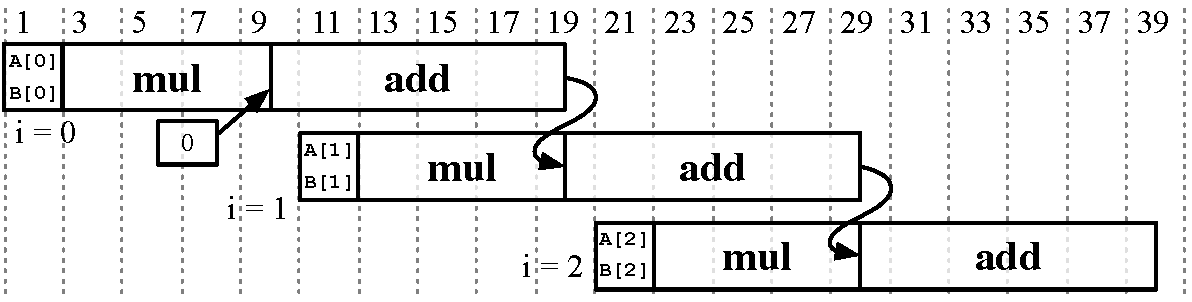
\includegraphics[width=0.8\linewidth]{bg/fig/schedule}
    \caption{%
        The resulting schedule of the example program in generated.
    }\label{bg:fig:schedule}
\end{figure}

Any valid schedule of this loop must satisfy the constraints imposed by
data-dependences.  For instance in our example, it is clear that in a
\emph{single} iteration, in the loop body, multiplication of \verb|A[i]|
and \verb|B[i]| must precede addition of \verb|d| and the multiplied
result.  Furthermore, in the $(i + 1)$-th iteration, access to the variable
\verb|d| must wait until \verb|d| is updated with a new value in the $i$-th
iteration, data-dependences therefore also exist on \verb|d| \emph{across}
loop iterations.  We call the former kind of dependences \emph{intra-iteration
dependences} and the latter \emph{inter-iteration dependences}.

Besides data-dependence constraints, the amount of resources available
also affects loop scheduling.  For instance, under our assumption in
Figure~\ref{bg:lst:dotprod} the RAM can only be read once per cycle, our
schedule thus should avoid reading from the same RAM in the same clock cycle.
We say a schedule is optimal, in the sense that the overall latency $L = (N -
1) \times \II + D$, is minimized, while none of the constraints are violated.
However with a much more complex program, finding the optimal schedule is
often an intractable task.  Limits on resource availability, along with
dependence constraints, make scheduling an NP-hard problem which is difficult
to solve optimally and efficiently~\cite{hwang91}.  In the following part
of this section, we discuss a heuristic technique known as \emph{modulo SDC
scheduling}~\cite{zhang13, canis14} used in LegUp to efficiently attack the
scheduling problem.


\subsection{Modulo SDC Scheduling}
\label{bg:sub:sdc}

Many algorithms exist that can schedule loops efficiently.  For example,
Fan~\etal~\cite{fan08} proposed that a schedule can be found by formulating
the constraints into a satisfiability modulo theory (SMT) problem and use
an SMT solver to modulo schedule operations.  A technique, Iterative Modulo
Scheduling (IMS)~\cite{rau94}, has been a widely adopted by compilers that use
software pipelining to schedule instructions for Very Long Instruction Word
(VLIW) processors~\cite{mcnairy03}.  This method has also been widely adopted
in HLS tools such as PICO-NPA~\cite{schreiber02}, Trident~\cite{tripp05} and
LegUp~\cite{canis13, canis14}.  IMS for software pipelining~\cite{rau94},
however did not consider operator chaining, \ie~allowing operations
with combinational logics to be carried out in the same clock cycle.
Schreiber~\etal~\cite{schreiber02} in their adoption of IMS in HLS, found
operator chaining to be non-trivial in IMS and requires static timing analysis
of combinational components~\cite{canis14}.  A new method, the modulo SDC
scheduling algorithm, has recently gained traction and has been used by
Canis~\etal~\cite{canis14} in their LegUp and Zhang~\etal~\cite{zhang13},
because an SDC formulation is more suited to model the effect of chaining
operators, and therefore in this subsection an overview is provided for their
modulo SDC scheduling approach.

\subsubsection{Constructing the Data-Dependence Graph}

In the first stage of modulo SDC scheduling, dependence relations are extracted
from the body of this loop.  These dependence relations form a dependence
graph, where vertices are operations, and edges between pairs of vertices
indicate dependence relations.  This dependence graph can subsequently be used
to derive data-dependence constraints.  Figure~\ref{bg:fig:depgraph} shows
the complete dependence graph of the loop in our Figure~\ref{bg:lst:dotprod}
example.
\begin{figure}[ht]
    \centering
    \begin{tikzpicture}
        \node (ai)  at (0,0) {\texttt{A[i]}};
        \node (bi)  [right=of ai, xshift=5mm] {\texttt{B[i]}};
        \node (mul) [below right=of ai, xshift=-5mm, yshift=5mm]
            {$\times$};
        \node (sum) [left=of mul, xshift=-10mm] {\texttt{d}};
        \node (add) [below right=of sum, xshift=-4mm, yshift=5mm] {$+$};
        \draw[->] (ai)  -- node[auto]{\pair10} (mul);
        \draw[->] (bi)  -- node[auto]{\pair10} (mul);
        \draw[->] (mul) -- node[auto]{\pair70} (add);
        \draw[->] (sum) -- node[auto]{\pair00} (add);
        \draw[->,dashed]
            (add) to[out=-135, in=180] node[left=3pt]{\pair{10}{1}} (sum);
    \end{tikzpicture}
    \caption{%
        The dependence graph formed by the data-dependences in the loop body
        of the dot-product example in Figure~\ref{bg:lst:dotprod}.  The dashed
        edge highlights the inter-iteration dependence.
    }\label{bg:fig:depgraph}
\end{figure}

Intra-iteration dependence edges in the graph are each labelled with $\langle
l, 0 \rangle$, a 2-tuple attribute of integers accordingly.  The first integer
$l$ signifies the number of clock cycles that must elapse between the start of
the predecessor and the successor operations.  The latter value $0$ indicates
that the dependence occurs in the same iteration.  To illustrate, the edge
between the multiplier ``$\times$'' and adder ``$+$'' has an attribute $\langle
7, 0 \rangle$, because ``$\times$'' takes 7 cycles to generate an output.

Additionally, inter-iteration dependences create elementary cycles in the
dependence graph.  For example, in each iteration the initial value of \verb|d|
depends on the final value of \verb|d| from the previous iteration.  In this
graph we thus add an edge from the output of the addition to the variable
\verb|d|.  We further describe that this dependence has a \emph{dependence
distance} of $1$, as $1$ iteration must elapse between the start of each pair
of value updates and its corresponding use.  This edge is then further assigned
an attribute $\langle 10, 1 \rangle$ which signifies that the adder has a
latency of $10$ cycles, and this dependence has a distance $1$.

\subsubsection{Finding the Minimum Initiation Interval}

Modulo SDC scheduling owes its efficiency to assuming an initial constant
$\II$ and attempting to search for a schedule that satisfies all constraints.
This search stops if a feasible schedule is found, otherwise $\II$ can be
incremented by 1 and search again until we discover a valid schedule.  To
begin with, we can find a lower bound on $\II$---which we call the minimum
initiation interval $\MII$, such that all schedules with an $\II$ less than
$\MII$ violate some constraints---as our initial constant $\II$.  The $\MII$ is
determined by both the inter-iteration dependences and resource limits.  For
each of the both types of constraints, an $\MII$ can be found, respectively
known as recurrence-constrained $\MII$ ($\RecMII$) and resource-constrained
$\MII$ ($\ResMII$)~\cite{rau94, canis14, zhang13}.  We first introduce methods
to compute both values, then the overall $\MII$ can then be computed using the
following equation:
\begin{equation}
    \MII = \max\left(\RecMII, \ResMII\right).
\end{equation}

Firstly, we compute $\ResMII$, by finding the most constrained resources
in the loop, as these limits impact the $\ResMII$ value.  For example, our
example in Figure~\ref{bg:lst:dotprod} does not impose limits on the number
of floating-point operators that can be allocated, but assumes there is a
constraint which restricts the rate of memory accesses, \ie~only one read is
allowed in each clock cycle.  Because each iteration requires two accesses to
the same memory, a $\ResMII = 2$ will thus fully occupy the RAM throughput.
To generalize this to all loops, we consider for each type of operations
$\opsymbol$ being used in the loop, the number of available resources
$r_\opsymbol$ for $\opsymbol$ and the number of occurrences $n_\opsymbol(G)$
of $\opsymbol$ in the loop dependence graph $G$, to evaluate $\left\lceil
n_\opsymbol(G) / r_\opsymbol \right\rceil$, the maximum ratio constitutes the
final $\ResMII$, or equivalently:
\begin{equation}
    \ResMII = \max_{\opsymbol~\in~\mathrm{OpTypes}}
        \left\lceil
            \frac{n_\opsymbol(G)}{r_\opsymbol}
        \right\rceil,
\end{equation}
where $\mathrm{OpTypes}$ is the set of all types of operations, \eg~array
accesses, arithmetic units, and others, used in the loop.

The second step is to evaluate $\RecMII$ by ensuring for all cycles $c$ in the
graph $G$ the following inequalities hold:
\begin{equation}
    \forall c \in \mathrm{Cycles}(G):
        \sum_{e \in c} \mathrm{lat}(e) - \II \times
        \sum_{e \in c} \mathrm{dist}(e) \leq 0,
\end{equation}
where $\mathrm{Cycles}(G)$ computes the set of all cycles in the graph $G$;
$e \in c$ enumerates all edges in the cycle $c$; and for an edge $e$ between
two vertices $v_1$ and $v_2$ of the form $v_1 \xrightarrow{\langle l, d
\rangle} v_2$, $\mathrm{dist}(e)$ and $\mathrm{lat}(e)$ respectively evaluate
to the latency $l$ and dependence distance $d$.  Hence, $\sum_{e \in c}
\mathrm{lat}(e)$ and $\sum_{e \in c} \mathrm{dist}(e)$ respectively sum
the latencies and dependence distances along all edges in the cycle $c$.
Equivalently, we can derive an equation for $\RecMII$ for the graph $G$:
\begin{equation}
    \RecMII = \max_{c~\in~\mathrm{Cycles}(G)}
        \left\lceil \frac{%
            \sum_{e \in c} \mathrm{lat}(e)
        }{%
            \sum_{e \in c} \mathrm{dist}(e)
        }
        \right\rceil.
\end{equation}
For example, in the dependence graph (Figure~\ref{bg:fig:depgraph}) of our
simple program (Figure~\ref{bg:lst:dotprod}), one cycle,
\tikz[baseline=-0.65ex]{%
    \node(d) at (0, 0) {\texttt{d}};
    \node(plus) at (5ex, 0) {$+$};
    \draw[->] (d)-- (plus);
    \draw[->,dashed] (plus) to[out=115, in=65] (d);
},
exists and the sums of latencies and dependence distances along this cycle are
$10$ and $1$ respectively, thus the $\RecMII$ of this graph is $\lceil 10 / 1
\rceil = 10$.

The simplest possible method of finding $\RecMII$ is therefore to enumerate
all cycles in the graph and compute the ratio between sums of latencies and
dependence distances.  Unfortunately in the worst case, the number of cycles
is exponential to the number of edges in a graph, this approach could become
intractable for large loops.  An alternative method based on the Floyd-Warshall
shortest path algorithm which runs in polynomial time, is thus proposed
in~\cite{rau94} to efficiently find $\RecMII$.  This method will be further
discussed in Chapter~\ref{chp:latopt}, Section~\ref{lo:sub:latency_analysis}.

\subsubsection{Scheduling Operations}

After assuming a tentative constant $\II$, in module SDC scheduling, we try to
construct an SDC problem in order to solve for the schedule.  We aim to assign
each operation, corresponding to each vertex $v$ in the graph, to a time slot
$s_v$ when it begins its operation.  While in this process, the scheduling
must ensure that all assignments do not violate data-dependence and resource
constraints.  For instance if a multiply operation is allocated with a time
slot in the second clock cycle, in each iteration it will start computation in
the second clock cycle of that iteration.

To begin, we ignore the resource limits for now and formulate an SDC
problem for the dependence constraints.  For each dependence edge $u
\xrightarrow{\langle l, d \rangle} v$ from vertex $u$ to vertex $v$ in the
graph, it is possible to write down the following inequality, where $s_u$ and
$s_v$ are respectively the time slots for vertices $u$ and $v$:
\begin{equation}
    s_u - s_v \leq \II \times d - l.
\end{equation}
For instance, the edge $\times \xrightarrow{\langle 7, 0 \rangle} +$ is an
intra-iteration dependence, hence $\II$ does not constraint the scheduling
relation between these two operations and we substitute $d$ with $0$ and $l$
with $7$, and the $\II$ term vanishes, to derive~\eqref{bg:eq:sdc_intra} below,
and the back-edge $+ \xrightarrow{\langle 10, 1 \rangle} \mathtt{d}$ produces
the following inequality in~\eqref{bg:eq:sdc_inter}:
\begin{align}
    s_\times - s_+ &\leq -7,
    \label{bg:eq:sdc_intra} \\
    s_+ - s_\mathtt{d} &\leq \II - 10.
    \label{bg:eq:sdc_inter}
\end{align}

Besides dependence constraints, additional constraints are used to limit the
length of critical paths in combinational logics, such that for instance, a
long chain of additions can be broken down into multiple cycles to guarantee
the frequency requirement.  For all paths $u \rightarrow \cdots \rightarrow
v$ between inter-iteration dependent vertices $u$ and $v$ consisting of
only combinational logics, it is possible to compute a critical path delay
$\mathrm{delay}(u, v)$.  This critical path delay is defined as the largest sum
of propagation delays of each intermediate operation along any combinational
path from $u$ to $v$.  For a pair of dependent vertices $u$ and $v$ such
that $\mathrm{delay}(u, v) > T_\mathrm{clk}$, where $T_\mathrm{clk} =
\frac{1}{f_\mathrm{clk}}$ and $f_\mathrm{clk}$ is the target clock frequency,
we can create the following constraint~\cite{cong06}:
\begin{equation}
    s_u - s_v \leq - \left\lceil
        \frac{
            \mathrm{delay}(u, v)
        }{
            T_\mathrm{clk}
        }
    \right\rceil + 1.
\end{equation}
This inequality ensures that for any the critical path delay between $u$
and $v$ greater than $T_\mathrm{clk}$, this path cannot be scheduled within
one clock cycle and it should be split into at least $ \left\lceil \frac{
\mathrm{delay}(u, v) }{ T_\mathrm{clk} } \right\rceil $ cycles.

Besides dependence and frequency constraints, Zhang~\etal~\cite{zhang13}
further introduces optional ones, such as lifetime constraints, which aim to
minimize the register requirements, and relative timing constraints, which can
be used to satisfy the timing requirement of user-specified I/O protocols.

The rationale of using the SDC formulation to model constraints is that
the feasibility of an SDC system and the corresponding solution, if it
exists, can be found efficiently.  More precisely, using the Bellman-Ford
algorithm~\cite{schrijver05}, it can run in $\Theta(l n)$ time, where
$l$ is the number of constraint inequalities and $n$ is the number of
variables~\cite{zhang13}.  Additionally, an SDC problem can be incrementally
solved, \ie~a new solution, if exists, can be updated in $O(m + n \log n)$
time when a constraint is added or removed, by using the algorithm presented
by Ramalingam~\etal~\cite{ramalingam99}.  In contrast, traditional ILP
scheduling techniques make use of $O(mn)$ variables to represent a scheduling
problem, where $m$ is the number of time slots and $n$ is the number of
operations~\cite{hwang91}, and solving this ILP problem often demands expensive
branch-and-bound procedures~\cite{zhang13} as ILP is NP-complete~\cite{karp10}.

Unfortunately, resources constraints, because of their non-linearity, cannot
be easily expressed as SDC constraints.  Therefore, a data structure called
\emph{modulo reservation table} (MRT) is used to keep track of resource
constraints as the loop is incrementally scheduled~\cite{canis14}.  The MRT
has $\II$ columns and each row tracks an available resource.  When a certain
resource is used in the time slot $s_u$, the MRT records an entry for this
resource in column $s_u \mod \II$ and the corresponding row of this resource.
To illustrate, consider our example in Figure~\ref{bg:lst:dotprod}, which
assumes a single read to the memory in one cycle for both arrays.  The MRT thus
has $\II = 10$ columns, and $1$ row for accessing the memory.  If \verb|A[i]|
is assigned with a time slot $0$, then a schedule assigning \verb|B[i]| to the
same time slot must be invalid, because a record exists for \verb|A[i]| in row
$1$ column $0$, and thus \verb|B[i]|, which is competing for the same resource,
hence must be scheduled in a later time slot.

A typical modulo SDC scheduling algorithm begins with a schedule without
resource constraints.  A priority function, is then used to sort all
resource-constrained operations by perturbation, which is to give greater
importance to operations that have a greater impact on the schedule when they
are moved~\cite{canis14}.  For each operator $u$ in this sorted list, if $u$ is
currently scheduled at time slot $t_u$ and does not have a resource conflict
in the MRT, a new constraint $s_u = t_u$ is constructed, otherwise a different
constraint $s_u \geq t_u + 1$ is used to ensure the operation $u$ is scheduled
one cycle later, so that it does not compete for the resource in time slot
$t_u$.  This newly created constraint is then tentatively added to the SDC
problem.  For a feasible resulting SDC problem, a new solution can be found
incrementally, otherwise the algorithm backtracks to a latest feasible SDC
formulation and try to schedule other operators before $u$.  A time budget can
also be used to limit the number of attempts to schedule resource-constrained
operators; if a valid schedule cannot be found under the given budget,
the $\II$ can be incrementing by $1$ to relax the dependence and resource
constraints, and the above mentioned procedure can be repeated until a valid
schedule is found.


\subsection{Obstacles in Adoption}
\label{bg:sub:obstacles_in_adoption}

High-level synthesis, with its development-cost advantage over traditional RTL
design paradigm, is gaining traction in the circuit design community.  It is
however in its early phase, and these tools still pose challenges in terms of
using them as early adopters.

HLS tools may have limited support for HLL constructs.  For instance,
Vivado HLS requires pointer arrays to reference values or arrays of values,
platform-specific functions such as \verb|memcpy()| and \verb|memset()|
are supported but \verb|const| values must be used, and finally, while
tail-recursive functions written with C++ template constructs can be
transformed into loops in compile time, recursion in general cannot be
implemented~\cite{vivado_hls}.  Additionally, software programs often rely
on libraries, many of which are platform-specific, whereas in HLS\@, these
libraries may not be appropriate and may likely be unavailable.  These above
limitations make migrating existing software source code to a functional HLS
design a demanding task.

Optimizing C code for HLS could be a laborious process and requires expertise
in hardware design.  Although software compilers face similar challenges
to make programs run faster, experienced software programmers can often
manually fine-tune software implementations for performance.  Because of
the flexibility of HLLs, currently it is difficult for designers to apply
common intuitions, and the quality of the synthesis result may be difficult
to predict~\cite{gupta04}.  Winterstein~\etal~\cite{felix13} implemented
K-means clustering algorithms in HLS, and discovered that with extensive
manual code transformations and \verb|#pragma| statements that are specific to
Vivado HLS, the tool can be persuaded to produce an efficient circuit.  When
compared to the RTL counterparts, their HLS designs achieved up to 40\% of
the performance in terms of area-time product.  Zhang~\etal~\cite{zhang15}
implemented a convolutional neural network (CNN) accelerator in Vivado HLS,
they optimized their design by program transformations techniques such as loop
interchange, tiling, pipelining and unrolling, and noticed that by enumerating
combinations of loop tile sizes, loop nest ordering and unroll factors, they
were able to select the best implementation by analytically estimating the
throughput of each.  Similarly, Suda~\etal~\cite{suda16} explored the design
space of their CNN accelerator by solving a resource-constrained throughput
optimization problem, in order to generate a high-performance CNN accelerator
to be synthesized in Altera OpenCL compiler~\cite{aoc}.  HLS tools can provide
some syntactic constructs to automate lower-level code transformations such
as instruction parallelism, loop pipelining and unrolling.  It is however up
to the engineer to decide how to utilize these transformations, and determine
if they will improve the design.  Higher-level optimizations such as the
manual design space exploration explained in earlier examples, may allow tools
to vastly improve the performance of HLS applications.  Automating these
techniques in HLS, however, remains a significant challenge.

HLS tools can often make use techniques such as loop pipelining discussed
in Section~\ref{bg:sub:sdc} to detect and exploit parallelism at the
instruction-level.  Coarser-grain parallelism, which is tightly associated with
the algorithmic details, is however much more complex~\cite{nane15}, and many
optimization opportunities are not yet exploited by HLS tools.  For instance,
unlike the CPU, which has a monolithic storage and thus their performance is
often limited by the memory wall, the FPGA has dedicated RAM blocks in the
logic fabric to distribute memory bandwidth via data reuse.  HLLs such as C
were designed with a mindset of the von Neumann architecture, and the source
code in C typically do not specify how the memory hardware is utilized.  For
this reason, HLS tools must be able to intelligently partition a monolithic
memory into smaller chunks that can be accessed in parallel, in order to
maximize performance; how to attain this is still a challenging research
area~\cite{cong11, cong12, wang13, felix15}.

Circuits produced by HLS tools are expected to be semantic-preserving.  It
means that they should be functional equivalent to the original C programs; in
other words, for any given program inputs, the tools should guarantee that the
computed outputs from the original C code and the synthesized circuit should
be identical.  A different class of optimizations, which we call \emph{lossy
optimization}, break this promise by optimizing data-paths in a way that may
impact numerical accuracy.  HLS tools could benefit from these optimizations
in the future, which bring further performance improvements that can not
be attained by traditional optimizations alone.  Because these approaches
could affect numerical accuracy, performance optimization and round-off error
analysis may be carried out simultaneously.  We will further discuss lossy
optimization methods such as expression balancing enjoyed by Vivado HLS and
LegUp in Section~\ref{bg:sec:discovering_equivalent_programs}.
% and word-length optimization in Section~\ref{bg:sec:wordlength}.
